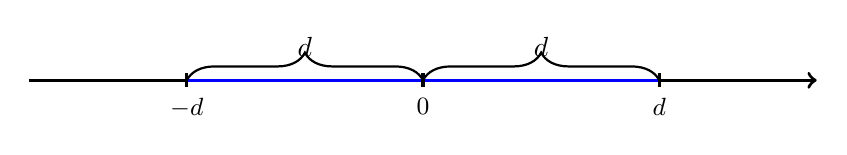
\begin{tikzpicture}
  \coordinate (A) at (-5,0);
  \coordinate (B) at (5,0);

  \coordinate (P) at (-3,0);
  \coordinate (Q) at (3,0);
  \coordinate (O) at (0,0);
  
  \draw [very thick,\lt->] (A) -- (B);
  \draw [very thick,blue] (P) -- (Q);
  
  \draw [very thick] (-3,2.5pt) -- +(0,-5pt) node [anchor=north, font=\small] {$-d$};
  \draw [very thick] (0,2.5pt) -- +(0,-5pt) node [anchor=north, font=\small] {$0$};
  \draw [very thick] (3,2.5pt) -- +(0,-5pt) node [anchor=north, font=\small] {$d$};

  \draw[thick,decorate,decoration={brace,amplitude=10pt},yshift=2.5pt] (P) -- (O) node [midway,above,yshift=5pt] {$\abs{d}$};
  \draw[thick,decorate,decoration={brace,amplitude=10pt},yshift=2.5pt] (O) -- (Q) node [midway,above,yshift=5pt] {$\abs{d}$};
\end{tikzpicture}
